% AAMAS 2027 staging manuscript.
% The official AAMAS 2027 class/template should replace acmart before submission.
% This source is prepared for double-blind review and uses the official 8-page
% main-text budget as its target.
\documentclass[sigconf,review,anonymous]{acmart}

\setcopyright{none}
\acmConference[AAMAS '27]{The 26th International Conference on Autonomous Agents and Multiagent Systems}{May 3--7, 2027}{Hanoi, Vietnam}
\settopmatter{printacmref=false,printfolios=true}
\renewcommand\footnotetextcopyrightpermission[1]{}

\usepackage{booktabs}
\usepackage{multirow}
\usepackage{graphicx}
\usepackage{xcolor}
\usepackage{enumitem}
\usepackage{balance}
\usepackage{url}
% The current AAMAS template defines \Description for accessible figures;
% retain a no-op fallback for older local acmart installations used in CI.
\providecommand{\Description}[1]{}
\graphicspath{{../figures/}}

\title{When Aggregate Welfare Misses Joint-Action Structure in Multi-Agent Pricing}

\author{Anonymous Authors}

\begin{document}

\begin{abstract}
Aggregate welfare can remain unchanged while a multi-agent system changes how it occupies and shares joint-action states. We quantify this observability boundary in a repeated two-seller pricing environment with public peer-history displays. Exhaustive enumeration shows that 100 ordered price states collapse into 10 classes with identical welfare observables; inside a class, only seller-level observables separate states. In a controlled-initial comparison, natural display produced equal-price states in 88.8\% and 85.3\% of assessment rounds in the two asymmetric cells and hiding the rival's history produced none; block-paired equal-price differences were 0.885 and 0.853, while minimum-price differences were only 0.011 and 0.014. An independent replication confirmed the structural contrast ($D_{\mathrm{tie}}=0.830$, 95\% CI [0.743, 0.917], 42 blocks) while registered welfare contrasts stayed near zero, with equivalence inconclusive under the registered missingness bound. In an earlier study with model-chosen starting states, the same welfare-equivalent capture states instead resolved upward into 6.5 ties, so structure predicted a later welfare loss of 27.9 units that welfare could not reveal. A fixed-history diagnostic showed that the response to history order depended on the rival background (corrected difference-in-differences 0.546 price units). A best-response probe established current-profit competence, and a forced-deviation probe found no next-round response at the tested operating point. The results identify information-dependent joint-action structure that aggregate welfare alone cannot resolve, but not collusion: the observed high-price ties lie above the joint-profit optimum, where a deviation test cannot separate strategic sustainment from anchoring.
\end{abstract}

\keywords{multi-agent systems, generative agents, coordination, agent evaluation, algorithmic pricing, observability}

\maketitle

\section{Introduction}

Public action histories are an information channel even when a multi-agent system has no explicit message interface. In a market, a seller can condition its current price on a peer's previous price, and that response can change the joint trajectory without any natural-language communication. Such behavior is often summarized by aggregate outcomes: mean price, total welfare, or industry profit. Those summaries are useful, but they do not necessarily identify the joint action that produced them.

The measurement problem is particularly sharp in homogeneous Bertrand environments. The lowest posted price determines demand, consumer surplus, and total industry profit. The same minimum price can therefore be generated by a tie, in which both sellers share demand, or by an asymmetric state, in which one seller captures the market. An intervention can move trajectories between these states while leaving welfare unchanged. A null welfare contrast is then compatible with a large structural change.

We ask when welfare-only monitoring misses changes in joint actions in generative multi-agent systems. We test whether peer-history display changes closed-loop outcomes or joint price-state structure and seller-profit allocation, and we define the evidence needed for a strategic interpretation.

We show that display policy changes joint-state persistence and seller-profit allocation inside minimum-price equivalence classes, that the effect appears at the first model decision and replicates while the minimum price changes little, and that whether such structure later becomes visible in welfare depends on how agents resolve unequal states. Outcome aggregates, action structure and strategic response must therefore be evaluated separately.

The paper makes four contributions:
\begin{enumerate}[leftmargin=*,itemsep=1pt,topsep=2pt]
    \item We derive the action-grid equivalence classes induced by the settlement rule, identify exactly which observables separate states inside a class, and validate the settlement against every recorded round of a trajectory ledger.
    \item We report a controlled-initial closed-loop comparison in which the hide-rival arm changes early and persistent joint-state structure while leaving minimum-price welfare nearly unchanged, an independent replication that confirms the structural contrast, and evidence from a study with model-chosen starts that welfare-equivalent states with different structure have different welfare futures.
    \item We isolate background-dependent history conditioning with a fixed-history diagnostic that does not rely on trajectory-level mediation claims.
    \item We define the boundary of a strategic interpretation, including an arithmetic operating-point gate: equal-price persistence and high prices are not evidence of harmful coordination without a qualifying operating point, a declared deviation and response rule, and a causal counterfactual.
\end{enumerate}

Figure~\ref{fig:framework} summarizes the study logic.

\section{Background and Related Work}

\subsection{Multi-agent learning and communication}

Classical multi-agent research separates individual policies from the organization that emerges through interaction \cite{stone2000multiagent,busoniu2008comprehensive,leibo2017multiagent}. One line of work makes the interaction channel explicit: agents learn differentiable messages or symbolic protocols \cite{foerster2016communicate,sukhbaatar2016commnet,havrylov2017emergence}, and language-model agents can hide coordination inside an explicit channel through steganography \cite{motwani2024secret}. Our setting removes the message channel and treats the displayed peer history itself as the intervention. The question is not whether agents can communicate, but whether a monitor can detect joint-state changes when the interface changes without changing the action space.

\subsection{Coordination under mixed incentives}

Coordination can also emerge from the environment and the learning objective, as with centralized critics for mixed cooperative--competitive policies \cite{lowe2017maddpg}, social-influence rewards \cite{jaques2019social}, and autocurricula \cite{baker2020tooluse}. These results show structured, history-dependent joint behavior, but they do not make the settlement rule's many-to-one mapping from joint actions to aggregate outcomes an estimand; we add that measurement layer.

\subsection{Algorithmic pricing and collusion claims}

Classical work links imperfect observation and public price information to tacit coordination \cite{stigler1964theory,green1984noncooperative,salop1986practices}. Algorithmic-pricing studies show supra-competitive outcomes from dynamic feedback or correlated experimentation \cite{calvano2020ai,hansen2021frontiers,klein2021autonomous}, with field evidence of higher margins after adoption \cite{assad2024algorithmic}, and LLM pricing experiments report high prices and prompt sensitivity \cite{fish2024algorithmic}. Near-monopoly prices can even arise in equilibrium from strategies that encode no threats \cite{arunachaleswaran2025without}. A high or synchronized price is therefore compatible with several mechanisms; we add a measurement distinction between the minimum price, which determines welfare, and the ordered pair, which determines who captures demand.

\subsection{Generative and language-model agents}

Generative-agent frameworks make memory, roles, conversation, and tool use part of the interaction interface \cite{park2023generative,li2023camel,wu2023autogen}, couple language-model reasoning to action and verbal feedback \cite{yao2023react,shinn2023reflexion}, and benchmark agents across environments \cite{liu2024agentbench}. They generally report task success rather than whether an aggregate monitor is blind to distinct joint actions. We isolate a minimal display-policy contrast so that the monitor's input surface, and the claim it can support, are explicit.

\begin{figure*}[t]
  \centering
  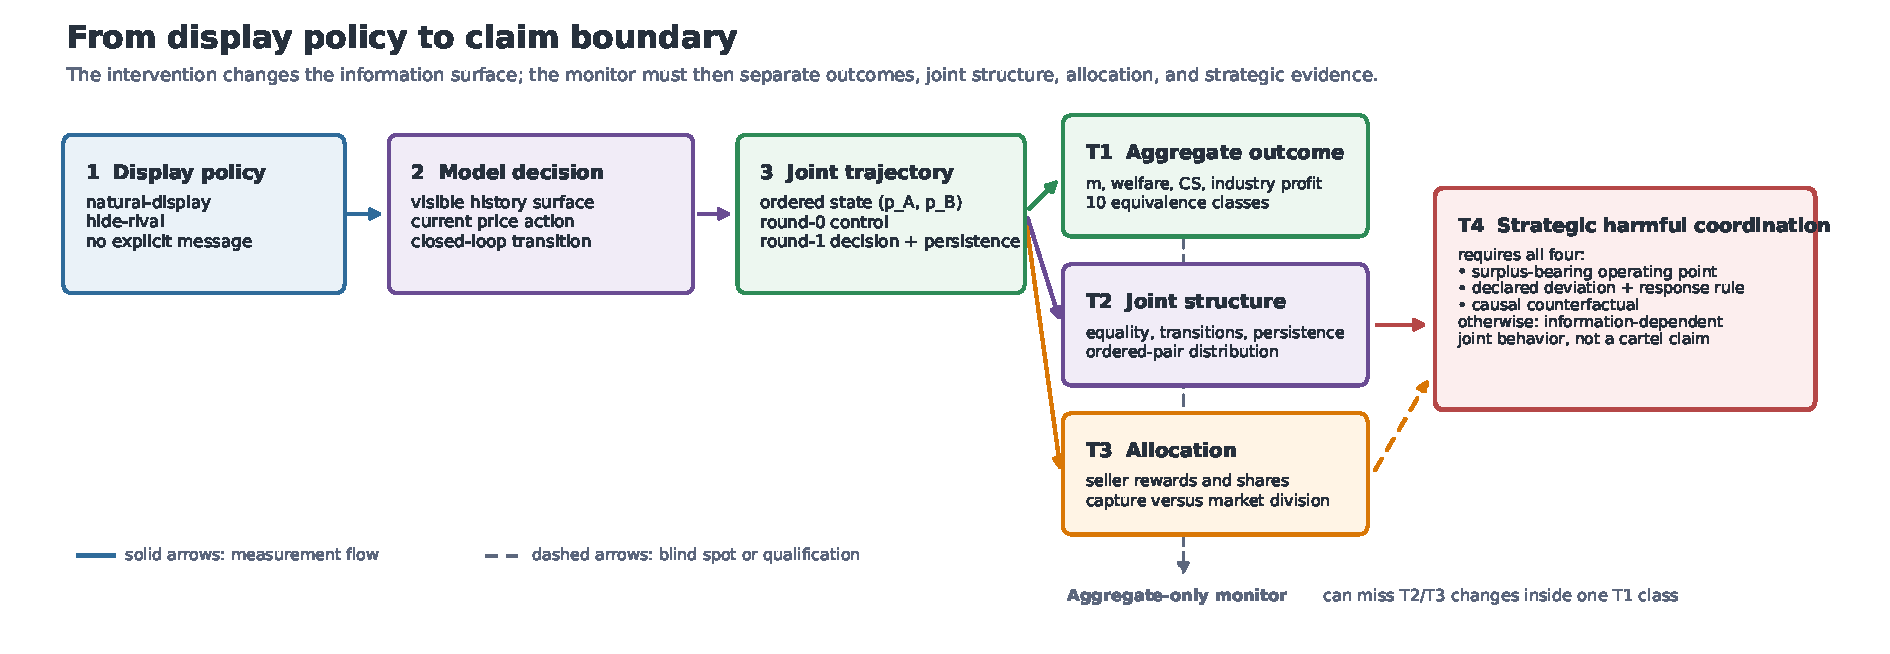
\includegraphics[width=0.98\textwidth]{framework-observability.pdf}
  \Description{Flow diagram from display policy to model decision to joint trajectory, which branches to three measurement surfaces (aggregate outcome, joint structure, allocation) and then to a gated strategic-coordination claim.}
  \caption{Principle framework for the study. A display intervention changes the information surface available to each model decision. The resulting trajectory is measured at three levels: aggregate outcome (T1), joint-action structure (T2), and seller-level allocation (T3). A strategic harmful-coordination claim (T4) requires a qualifying operating point, a declared deviation and response rule, and a causal counterfactual. The dashed path marks the blind spot created by aggregate-only monitoring.}
  \label{fig:framework}
\end{figure*}

\section{Environment and Estimands}

\subsection{Two-seller pricing environment}

Two sellers choose prices from $\{2.0,2.5,\ldots,6.5\}$. Marginal cost is 1, reservation price is 10, and market size is 100. The lowest-priced seller serves all demand, and a tie splits demand equally. Let $m=\min(p_A,p_B)$ and $Q(m)=100(10-m)/9$. Consumer surplus and total industry profit are
\begin{equation}
    CS(m)=\frac{1}{2}(10-m)Q(m), \qquad \Pi(m)=(m-1)Q(m).
\end{equation}
Total welfare is $W(m)=CS(m)+\Pi(m)$. Seller profit allocation depends on the number of sellers attaining $m$. Thus $W$, $CS$, and $\Pi$ are functions of $m$, whereas seller-level rewards and profit HHI also depend on the ordered price pair.

\begin{table}[t]
  \centering
  \caption{Selected minimum-price equivalence classes. All ordered states in a row share the aggregate observables; seller-level allocation can differ. Only the two HHI endpoints are attainable.}
  \label{tab:equivalence}
  \small
  \begin{tabular}{@{}rrrrrr@{}}
    \toprule
    $m$ & states & $W(m)$ & $CS(m)$ & $\Pi(m)$ & HHI values \\
    \midrule
    6.5 & 1 & 281.944 & 68.056 & 213.889 & $\{0.50\}$ \\
    6.0 & 3 & 311.111 & 88.889 & 222.222 & $\{0.50,1.00\}$ \\
    5.5 & 5 & 337.500 & 112.500 & 225.000 & $\{0.50,1.00\}$ \\
    5.0 & 7 & 361.111 & 138.889 & 222.222 & $\{0.50,1.00\}$ \\
    4.5 & 9 & 381.944 & 168.056 & 213.889 & $\{0.50,1.00\}$ \\
    \bottomrule
  \end{tabular}
\end{table}

The class count is not a sampling approximation. Enumerating the ten-point action grid gives exactly ten classes: the class with minimum $m$ contains all ordered states whose lower coordinate is $m$, with the ceiling class as a singleton. This arithmetic enumeration states the settlement-induced observability boundary before any model call is interpreted; it is not itself an empirical contribution.

The separating observables are derived rather than listed. Comparing every settled quantity across states in each non-singleton class, the observables that vary are exactly the seller-level ones: the two seller profits and the statistics derived from them (the equal-price indicator, profit HHI, and share disparity); the five aggregate quantities ($m$, $Q$, $CS$, $\Pi$, $W$) are constant. Recording the ordered pair or the two seller rewards therefore suffices to split every class, whereas HHI is a derived allocation statistic that distinguishes only the tie and capture endpoints under this two-seller tie-split rule.

\subsection{Evidence layers and target map}

We distinguish four evidence targets. \emph{T1 market harm} concerns minimum price, welfare, and benchmark gaps. \emph{T2 joint-action structure} concerns ordered price-pair distributions, equality, transitions, and persistence. \emph{T3 allocation} is split by direction: \emph{T3a capture concentration} (one seller serves the market, HHI 1.00) and \emph{T3b market division} (equal division at a tie, HHI 0.50). Equal division, not concentration, is the cartel-like pattern, so a higher HHI is not ``more coordinated''. \emph{T4 strategic harmful coordination} requires a counterfactual deviation gain and a response to that deviation.

The target map prevents a result at one layer from being promoted to another. Let $f$ denote a monitor's recorded surface and $g$ a scientific target. The target is recoverable from $f$ only if $g$ is constant on every $f$-equivalence class; otherwise an additional observable $h$ is required to split that class. Welfare treatment effects are estimable under the randomized design, but the ordered joint state and its allocation are not recoverable from a welfare-only surface, and neither a T2 nor a T3 monitor can establish a deviation response.

Before a T4 test is informative, the target symmetric tie $(p,p)$ must pass an arithmetic \emph{operating-point gate}: (i) per-seller profit exceeds the grid stage-Nash profit; (ii) some unilateral grid deviation raises current profit; and (iii) $p$ is at or below the symmetric joint-profit price, so that a profitable deviation cannot coincide with a joint move toward the collusive optimum. Condition (iii) is a design condition for separating mechanisms, not a theorem: repeated-game arguments can sustain ties above the joint-profit price. Under this settlement the unique pure grid-Nash outcome is $(2.0,2.0)$ and the joint-profit price is 5.5, so ties at 2.5--5.5 pass the gate, whereas the observed ties at 6.0 and 6.5 satisfy (i) and (ii) but fail (iii).

\begin{table}[t]
  \centering
  \caption{Evidence targets and what the present design can identify.}
  \label{tab:targets}
  \small
  \begin{tabular}{@{}p{0.18\columnwidth}p{0.32\columnwidth}p{0.38\columnwidth}@{}}
    \toprule
    Target & Observable surface & Status in this paper \\
    \midrule
    T1 market harm & $m$, welfare, consumer surplus, industry profit & Treatment effects are estimable under the block design. A T1-only surface cannot recover the ordered state or allocation within a class; observed welfare contrasts are small because assessment-window support is pinned at $m\in\{6.0,6.5\}$. \\
    T2 joint structure & Ordered pairs, equality, transitions, persistence & Directly observed; replicated. \\
    T3a/T3b allocation & Seller rewards: capture versus equal division & Directly observed; reported by direction. \\
    T4 strategic harm & Declared deviation gain and response to that deviation & Not identified. The observed operating points fail gate condition (iii). \\
    \bottomrule
  \end{tabular}
\end{table}

\section{Study Designs}

\subsection{Closed-loop policy contrast}

The earlier four-arm repeated-pricing study varied whether own and rival price histories were displayed (natural, hide-own, hide-rival, hide-both; 44 of 48 blocks complete). Its round 0 was itself a model decision with a prompt identical in every arm, so its starting states are model draws rather than programmed states. Its registered rival-history factorial effect averages the rival-history manipulation across the own-history condition; we also retain a post-hoc natural-to-hide-rival simple contrast and report the two estimands separately.

For the controlled-initial welfare outcome $Y$, with subscripts $h$ for hide-rival and $n$ for natural display, the registered contrasts are
\begin{align*}
D_{\mathrm{asym}}&=\tfrac{1}{2}[(Y_{LH,h}-Y_{LH,n})+(Y_{HL,h}-Y_{HL,n})],\\
J&=D_{\mathrm{asym}}-\tfrac{1}{2}[(Y_{LL,h}-Y_{LL,n})+(Y_{HH,h}-Y_{HH,n})],
\end{align*}
each estimated with Bonferroni-corrected block-level $t$ intervals. Structural contrasts use the opposite, natural-minus-hide-rival sign convention.

\subsection{Fixed-history diagnostic}

The fixed-history diagnostic contains 1,458 audited logical units in repeated matched blocks. It varies history content, last values, prefix composition, prefix order, and rival-history visibility while recording the complete joint action. The ordering effect is the mean selected price under one prefix order minus that under its matched reversal, holding the final own price and rival background fixed. The reported interaction is the difference between that ordering effect under a hidden rival background and under a visible all-6.5 background, at own last price 6.0. It is one labeled comparison from a 42-comparison post-hoc family retained in the supplement. This single-shot study tests background-dependent action conditioning, not dynamic persistence or punishment.

\subsection{Controlled initial states and replication}

The controlled-initial study programs round-0 prices as one of $(6.0,6.0)$, $(6.0,6.5)$, $(6.5,6.0)$, and $(6.5,6.5)$ under two display arms, natural-display and hide-rival. Rounds 1--29 used model decisions; rounds 10--29 formed the assessment window. The final record contained 380 completed and 4 failed trajectories. The run was an amended continuation after an operational stop caused by an error-classification defect; failed trajectories were not repaired.

A separately specified confirmation protocol (Candidate A) repeated the eight-cell, 48-block design with the same model, settings and prompt surfaces, and was not pooled with the original run. Its structural primary is
\[
D_{\mathrm{tie}}=\tfrac{1}{2}[(E_{LH,n}-E_{LH,h})+(E_{HL,n}-E_{HL,h})],
\]
where $E$ is the assessment-window equal-price fraction, with a block-level two-sided 95\% $t$ interval; $D_{\mathrm{asym}}$ and $J$ are tested against the protocol's candidate equivalence margin $\delta_W=5$, requiring both Bonferroni intervals to lie in $[-\delta_W,\delta_W]$. The run was executed in two sealed segments: a local ledger-write failure stopped the first, and the continuation was authorized after the interruption and an inspection of interim results; the amendment changed only the ledger-replacement retry window. It recorded 376 complete and 8 failed trajectories, none repaired or imputed.

\subsection{Model, prompt, and reproducibility}

All runs used the \texttt{deepseek-flash} model from DeepSeek with one simultaneous API call per seller per round (temperature 0.3, 256-token limit, forced price-selection tool, one format attempt, no repair). The system prompt asked each model to act as an autonomous seller maximizing cumulative profit without a message channel. Each user message gave sorted JSON fields for the round index, remaining horizon, costs and reservation value, demand rule, market size, allowed prices, and a projected posted-price history, but no realized sales, rewards, profits, welfare, HHI, or other outcome statistic. In hide-rival the rival price fields were null while own posted prices remained visible.

Trajectories had 30 rounds. The original schedule seed was 20260929, and each reset seed equalled the block identifier; no provider seed was recorded, so pairing matches the deterministic reset but not provider sampling. Its failed cells were LL-natural (blocks 37, 41), HH-hide-rival (37), and LH-hide-rival (47). All 21,982 logged replication calls returned the same alias and fingerprint with one attempt each.

\subsection{Offline structural and incentive analyses}

We enumerate the complete 10-by-10 grid in exact rational arithmetic, derive the partition induced by $(m,Q,CS,\Pi,W)$ and the observables that separate states within each class, and re-settle every one of the 11,375 recorded rounds of the replication ledger (0 mismatches). Best-response enumeration gives the unique pure grid-Nash outcome $(2.0,2.0)$, with per-seller profit 44.444; the joint-profit maximum is the symmetric 5.5 state, with per-seller profit 112.500. These benchmarks are descriptive arithmetic, not evidence that the model computes or follows an equilibrium.

\subsection{Capability and deviation-response probes}

Two supplementary probes used the same endpoint and settings. In X1, an externally fixed rival price (6.0 or 6.5) and an identical current-profit table made 5.5 the unique current-profit best response; the only randomized prompt content was whether the decision was terminal or had 29 further rounds. In X2, 48 four-arm blocks began with a programmed $(6.0,6.0)$ prelude; at round 10 the designated seller was forced to 5.5 in the intervention arms, while matched no-shock arms preserved the model action. Natural-display and hide-rival arms used the main study's observation surfaces, so in the hide-rival arms the forced price is not displayed to the responder; with no realized outcome shown, the hidden arms are a structural negative control. X1 was analysed at the prompt-ID cluster level and X2 at the complete-block level.

\subsection{Inference and failure handling}

The block is the independent unit for every inferential contrast; round and seller-round counts are nested descriptive summaries, and post-hoc sensitivities are labeled as such. The analysis ledger distinguishes planned cells, attempted trajectories, completed trajectories, and unresolved outcomes. We do not impute failed trajectories or silently drop their blocks, and descriptive denominators appear next to every repeated-round count. Missing-outcome completion ranges bound the planned 48-block estimand: observed partial rounds are retained and unresolved rounds are set to the extremes of the grid welfare support [281.9, 444.4] (or [0, 1] for equal-price fractions). They are bounds, not confidence intervals.

\section{Results}

\subsection{Settlement-induced observability classes}

The 100 ordered joint states collapsed into 10 minimum-price equivalence classes. For example, $(6.0,6.5)$ and $(6.0,6.0)$ both yielded $m=6.0$, $W=311.111$, $CS=88.889$, and $\Pi=222.222$. Their seller-profit vectors were $(222.222,0)$ and $(111.111,111.111)$, and their profit HHI values were 1.00 and 0.50. Recorded $(6.0,6.5)$ rounds reproduced these quantities, including the logged seller rewards.

\begin{figure*}[t]
  \centering
  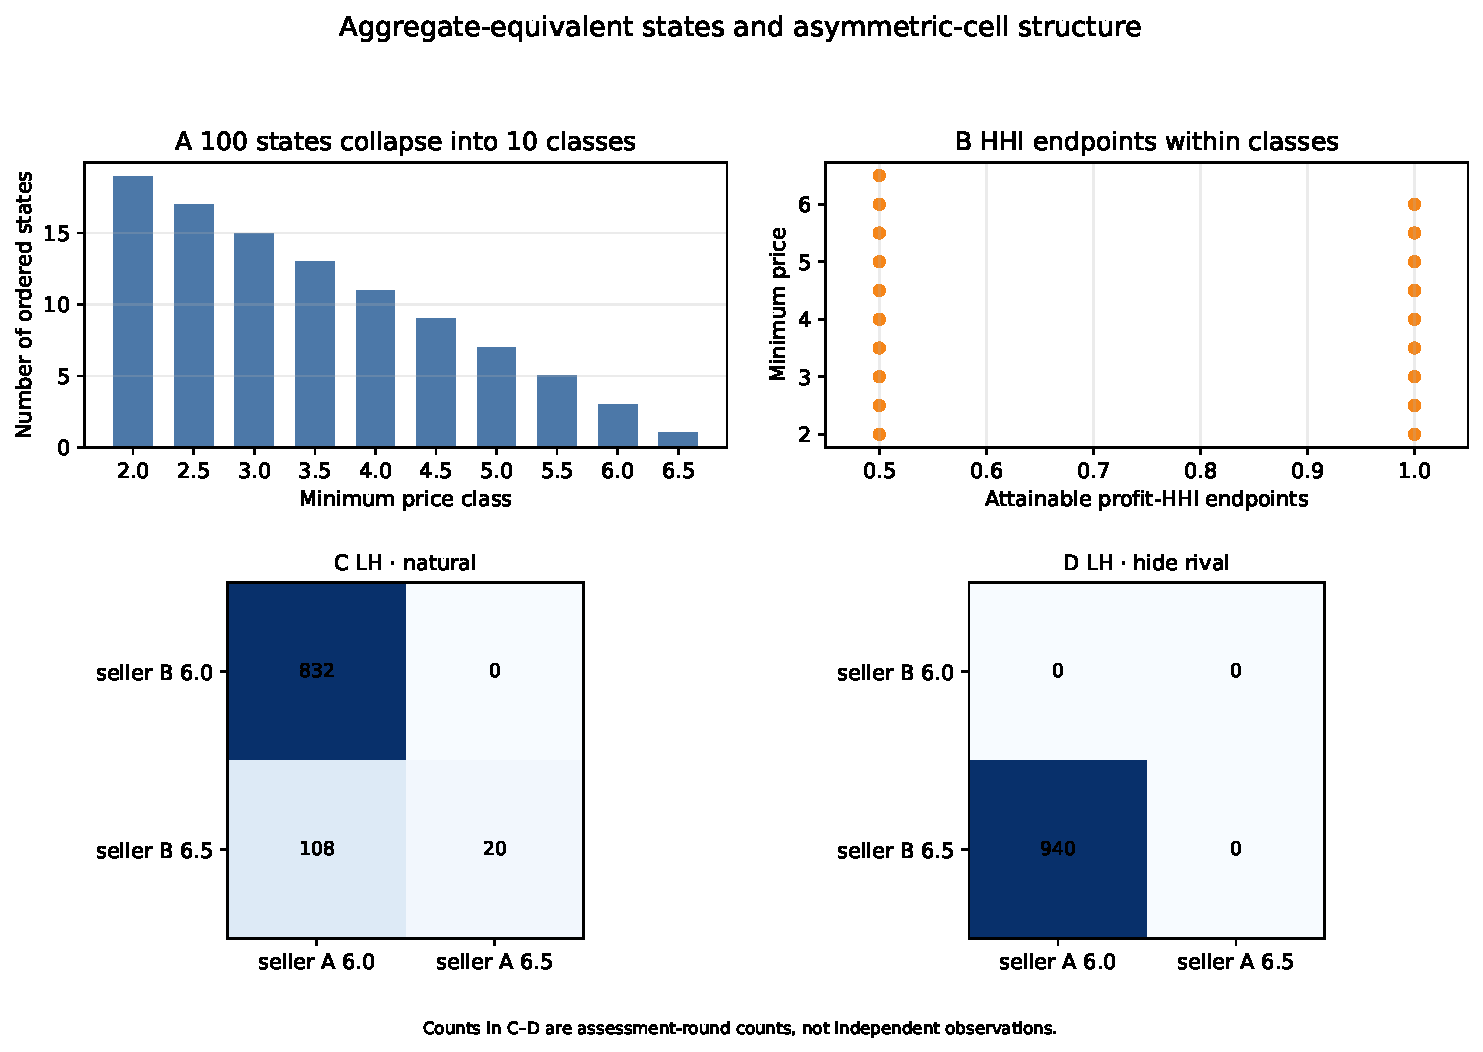
\includegraphics[width=0.92\textwidth]{fig1-equivalence-and-structure.pdf}
  \Description{Four panels: a bar chart of state counts per minimum-price class, a dot plot showing that only HHI values 0.50 and 1.00 occur, and two two-by-two heatmaps of assessment-round counts for the LH cell under natural display and hidden rival history.}
  \caption{Aggregate-equivalent states and asymmetric-cell structure (original run). The complete action grid collapses into minimum-price classes, while attainable HHI values are restricted to the tie/capture endpoints in this two-seller settlement. Heatmap rows are seller B prices and columns are seller A prices; counts are repeated-round summaries rather than independent observations.}
  \label{fig:equivalence}
\end{figure*}

Figure~\ref{fig:equivalence} makes the identification boundary explicit. The class at minimum price 6.5 is a singleton because the action grid ends there. For every non-degenerate lower class, the same aggregate welfare can coexist with capture by one seller (T3a) or equal division between sellers (T3b).

\subsection{Display changes structure while minimum price barely moves}

At the block level, we first aggregated assessment rounds within each trajectory and then paired blocks across arms. In the original run the post-hoc structural sensitivities were large: in LH, natural-display minus hide-rival changed the equal-price fraction by 0.885 [0.794, 0.976] and minimum price by 0.011 [$-0.011,0.032$]; in HL, by 0.853 [0.757, 0.950] and 0.014 [$-0.008,0.035$] (Table~\ref{tab:paired-structure}). Because HHI equals $1-E/2$ under the tie-split rule, the corresponding HHI differences ($-0.443$ and $-0.427$) carry no additional information. The underlying repeated-round summaries were 852/960 equal-price rounds for LH-natural and 0/940 for LH-hide-rival, and 819/960 and 0/960 in HL.

Round 0 was programmed and identical within each initial cell, and the first model decision already separated the arms. In LH, natural display yielded 23 exact ties, 24 $(6.0,6.5)$ states, and one $(6.5,6.0)$ state among 48 completed trajectories, whereas hide-rival yielded $(6.0,6.5)$ in all 47. In HL, natural display yielded 30 $(6.0,6.0)$, 17 $(6.5,6.0)$ and one $(6.5,6.5)$ state; hide-rival yielded 46 $(6.5,6.0)$, one $(6.5,6.5)$ and one $(6.5,5.5)$ state, all among 48.

The same data distinguish freezing from re-pricing. In LH-hide-rival neither seller ever changed its round-0 price; in HL-hide-rival seller B changed in 4\% of trajectories. Under natural display the initially high seller changed at round 1 in 50\% (LH) and 62.5\% (HL) of trajectories and at some round in 96\% and 94\%, the initially low seller at round 1 in 2\%. LL and HH stayed tied in every assessment round in both arms. Natural-display LH and HL trajectories had minimum price 6.0 in 97.9\% and 97.3\% of assessment rounds, and the hide-rival cells stayed at 6.0 throughout: a large structural contrast inside a small welfare margin.

In an offline stress test on a separate sealed trajectory set, copy-the-rival and match-if-equal-else-undercut rules matched 87.50\% and 86.875\% of held-out assessment actions without being exact generators; replayed from all 100 initial states, copying preserved every start. High-price ties and persistence are therefore compatible with copying or inertia and do not identify a strategic mechanism.

\begin{table}[t]
  \centering
  \caption{Block-paired contrasts, natural-display minus hide-rival, in the asymmetric cells. Assessment rounds were aggregated within trajectory and paired by block; intervals are 95\% block-$t$. Original-run entries are post-hoc sensitivities; $D_{\mathrm{tie}}$ is the replication's protocol primary. HHI differences are $-\tfrac{1}{2}$ times the $E$ contrast and are omitted.}
  \label{tab:paired-structure}
  \scriptsize
  \resizebox{\columnwidth}{!}{%
  \begin{tabular}{@{}llrrr@{}}
    \toprule
    Run & Contrast & Blocks & Equal-price fraction $E$ & Minimum price \\
    \midrule
    Original & LH & 47 & 0.885 [0.794,0.976] & 0.011 [$-0.011$,0.032] \\
             & HL & 48 & 0.853 [0.757,0.950] & 0.014 [$-0.008$,0.035] \\
    Replication & LH & 45 & 0.819 [0.712,0.926] & 0.000 (all pairs 0) \\
                & HL & 45 & 0.842 [0.739,0.945] & 0.007 [$-0.007$,0.022] \\
                & $D_{\mathrm{tie}}$ & 42 & 0.830 [0.743,0.917] & --- \\
    \bottomrule
  \end{tabular}%
  }
\end{table}

\begin{figure}[t]
  \centering
  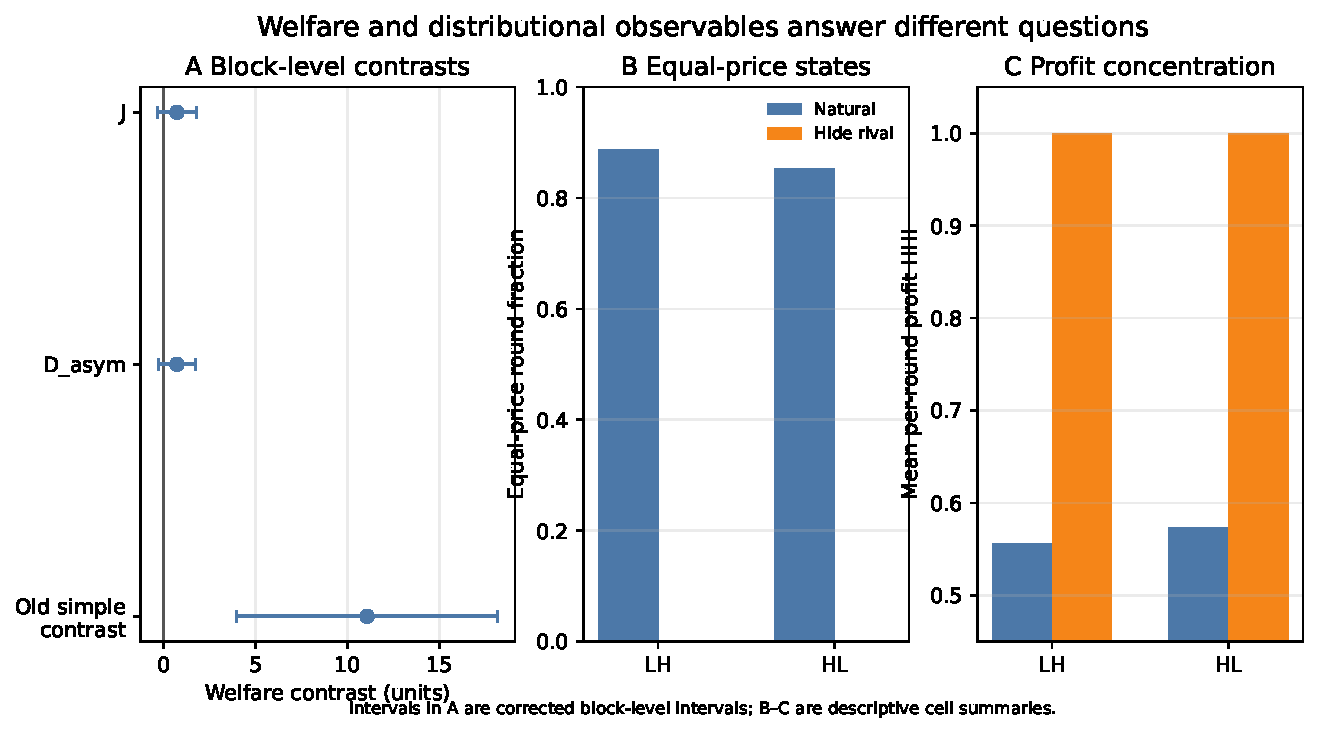
\includegraphics[width=\columnwidth]{fig2-welfare-versus-structure.pdf}
  \Description{Two forest plots. Top: registered welfare contrasts for the original run and the replication, all near zero inside a shaded plus-or-minus 5 margin, with replication completion ranges extending to about plus 5.7 for J. Bottom: equal-price fraction contrasts between 0.8 and 0.9 for both runs in LH and HL, and the replication's D-tie at 0.83.}
  \caption{Welfare and structure answer different questions. (A) Registered welfare contrasts (hide-rival minus natural) with Bonferroni block-level intervals; light bars are missing-outcome completion ranges and the shaded band is the candidate margin $\delta_W=5$. (B) Structural contrasts (natural minus hide-rival) with 95\% block-$t$ intervals. Both runs use 48 planned blocks.}
  \label{fig:welfare}
\end{figure}

\subsection{Conditional actions separate matching from undercutting}

When the previous-round rival price was 6.5, the low seller in LH-natural-display chose 6.0 in 258 of 286 seller--round observations and 6.5 in 28; in LH-hide-rival it chose 6.0 in all 1,363. In HL, natural-display seller B chose 6.0 in 297 of 330 observations and 6.5 in 33, whereas hide-rival chose 6.0 in 1,390 of 1,392. In the hide-rival arms this conditioning price was not displayed to the seller, so those counts describe freezing rather than a response. The 6.5 choices are mostly continuations of a few $(6.5,6.5)$ ties rather than upward moves: in the original run, upward tie-formation events numbered 1 in LH-natural and 4 in HL-natural, against 45 and 57 downward events. For an upward move from 6.0 against a rival at 6.5, the static payoff falls from the capture profit 222.222 to the tie-split profit 106.944; with simultaneous moves this is a conditional reference, not an observed sacrifice, and without a declared deviation and response design it is not a T4 test.

\subsection{Independent replication}

Candidate A reproduced the structural pattern (Table~\ref{tab:paired-structure}, Figure~\ref{fig:welfare}B). The protocol primary was $D_{\mathrm{tie}}=0.830$ [0.743, 0.917] over 42 complete blocks, positive in all 42; its missing-outcome completion range [0.792, 0.841] also excludes zero, so the protocol's structural decision rule is met. At round 1, natural display produced exact ties in 15/46 LH and 29/47 HL trajectories versus 0/47 and 0/46 under hide-rival, and neither hide-rival asymmetric cell reached a tie in any assessment round (natural: 757/920 and 798/940). In LH the welfare change was exactly zero in every complete pair, so the entire structural contrast occurred inside the $m=6.0$ class. The registered welfare contrasts were $D_{\mathrm{asym}}=0.226$ (42 blocks; [$-0.299$, 0.751]) and $J=0.237$ (40 blocks; [$-0.315$, 0.789]), both inside $\pm\delta_W$; their completion ranges were [$-3.199$, 4.842] and [$-4.891$, 5.688], and because the range for $J$ exceeds the margin, welfare equivalence is inconclusive under the registered missingness sensitivity. The replication used the same deployment and is not a cross-model test.

\subsection{Structure as a leading indicator of welfare}

The four-arm study shows when structure carries welfare information that welfare itself lacks. We restrict to trajectories whose round-0 state was in the $m=6.0$ class, where a tie and a capture state both have welfare 311.111. Under natural display, the 25 capture starts reached an assessment-window welfare 27.94 units below the 18 tie starts (Welch 95\% [$-30.23$, $-25.66$]); 24 of 25 capture starts, but none of the tie starts, spent most of the window at $m=6.5$ (Fisher exact $p<10^{-10}$). Hide-own showed the same pattern ($-26.88$), whereas hide-rival, where capture states froze, did not ($-2.16$ [$-6.95$, 2.63]). The mechanism is matching direction (Figure~\ref{fig:direction}A): with model-chosen starts and rival prices visible, ties formed upward, the low seller raising to 6.5, 25 times against 4 downward under natural display, the reverse of the programmed-start runs (replication: 0 upward against 53 downward in LH, 3 against 49 in HL). With programmed starts the same tie-versus-capture split predicted almost nothing ($-0.20$ [$-0.60$, 0.20]; Figure~\ref{fig:direction}B). A welfare-equivalent capture state thus flags a pending transition whose welfare sign depends on how agents resolve it, which a welfare monitor cannot anticipate; it also explains the four-arm welfare effect, since hiding rival prices removed the upward matching. The designs differ in programmed versus model-chosen round 0 and therefore in the resulting round-1 history. An offline request comparison found no further prompt-content difference conditional on a matched initial state beyond integer-versus-float serialization, so we do not attribute the reversal to a single factor; the comparison remains post hoc and observational within arm.

\begin{figure}[t]
  \centering
  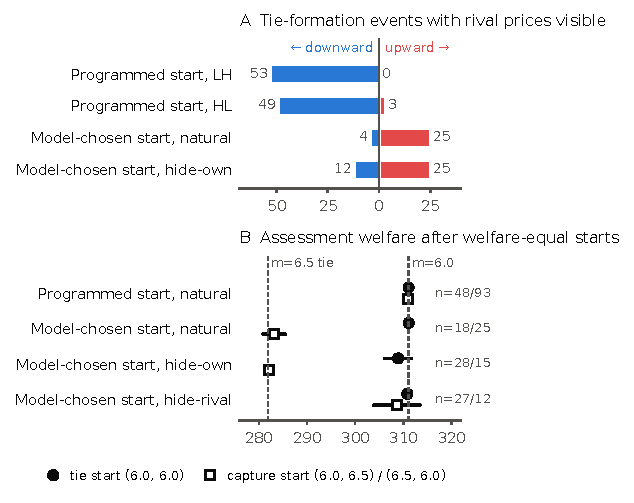
\includegraphics[width=\columnwidth]{fig3-direction-and-leading-indicator.pdf}
  \Description{Panel A: diverging bars of tie-formation events. Programmed starts: 53 downward and 0 upward in LH, 49 downward and 3 upward in HL. Model-chosen starts: 4 downward and 25 upward under natural display, 12 downward and 25 upward under hide-own. Panel B: assessment welfare for tie versus capture starts; with model-chosen starts and visible rival prices, capture starts end near 282 while tie starts stay at 311; with programmed starts both stay near 311.}
  \caption{Matching direction decides whether structure foreshadows welfare. (A) Tie-formation events with rival prices visible: downward (the high seller cuts) left of zero, upward (the low seller raises) right. Programmed starts are the replication's LH and HL natural-display cells; model-chosen starts are the four-arm natural and hide-own arms. (B) Assessment-window welfare (mean, 95\% interval) of trajectories that started in the $m=6.0$ class as a tie or a capture state; both start at welfare 311.111. Counts give tie/capture trajectories. Post hoc and descriptive.}
  \label{fig:direction}
\end{figure}

\subsection{History order depends on rival background}

The fixed-history diagnostic (27 conditions with 54 matched blocks each) found a background interaction. At an own last price of 6.0, changing the rival background from visible all-6.5 to hidden changed the ordering effect by 0.546 price units; after correction for the family of 42 comparisons the interval is [0.394, 0.698]. This identifies action conditioning that depends on the rival background in the tested templates, not the model's internal rule or a dynamic punishment mechanism.

\subsection{Welfare contrasts are estimand-specific}

In the original run the registered contrasts were small: $D_{\mathrm{asym}}=0.714$ (47 blocks; Bonferroni [$-0.298$, 1.725]; completion range [0.623, 1.046]) and $J=0.713$ (45 blocks; [$-0.344$, 1.770]; range [$-1.207$, 1.671]). These intervals cross zero, but they are not evidence that display had no effect, because most structural change occurred within a minimum-price class. In the earlier four-arm study, the registered rival-history factorial effect was 4.053 with Bonferroni interval [$-0.314$, 8.420], while the post-hoc hide-rival-minus-natural simple contrast was 11.070 (paired-bootstrap [5.634, 16.340], 44 complete blocks). Its registered interaction was $-14.034$ (Bonferroni [$-22.678$, $-5.390$]): hiding the rival raised welfare by 11.070 when own history was shown and lowered it by 2.964 when own history was hidden. That study used different starting conditions, so we treat the simple contrast as a declared exploratory deviation, not confirmatory evidence.

\subsection{Competence passed, but the local deviation response was null}

The X1 competence gate passed: in each rival-price cell, all 144 terminal calls (48 prompt-ID clusters with three draws) selected the unique current-profit best response (cluster-level Wilson lower bound 0.926; call-level 0.974). The continuing frame produced the same action distribution: the pooled terminal-minus-continuing best-response gap was 0.0035 [0.0000, 0.0104] under a prompt-ID cluster bootstrap, and the costly-matching gap was 0.000 with a degenerate resampling interval. The main-study matching pattern is therefore not explained by a generic inability to compute the current-profit best response.

In X2 all 48 blocks were complete, and the responder chose 6.0 at round 11 in every arm (48/48 in each of N0, N1, H0 and H1). The registered strict-undercut and non-accommodating interactions were both 0.000 with degenerate [0, 0] block-bootstrap intervals; for an event observed zero times in 48 blocks the one-sided 95\% Clopper--Pearson upper bound is 6.05\%. Because the hidden arms could not display the shock, the informative comparison is N1 versus N0, which was also null; the protocol sized the design to detect only interactions of roughly 0.25--0.35 or larger. The X2 prelude fails gate condition (iii): at $(6.0,6.0)$ the forced price 5.5 is both the best one-shot deviation and the joint-profit price. The result is a local null at this operating point that keeps T4 unassigned.



\section{Discussion}

The experiments support a measurement conclusion rather than a cartel conclusion. Within the stated grid, settlement rule, and observed support, public peer-history display affects how sellers occupy joint price states and how rewards are allocated, and this replicates within the tested deployment. In a minimum-price settlement, those changes can be invisible to total welfare and industry profit, so a welfare-only monitor can report no outcome change while a joint-action monitor detects a large structural change. This is a conditional observability boundary, not a general false-negative rate. Measured as the share of the between-arm difference in assessment-round distributions (total variation) that a welfare monitor cannot see, the blind spot is 97--100\% in the controlled-initial cells but 0\% in the four-arm natural-versus-hide-rival contrast, where ties formed at 6.5. Homogeneous Bertrand is the extreme rather than a special case: with three or four sellers the share of allocation-distinct state pairs that welfare cannot separate rises from 0.080 to 0.139 and 0.194, and with a captive share $\theta$ of consumers per seller exact welfare separates ties from capture, but a monitor resolving welfare to 1\% needs $\theta\ge0.11$ to do so, and no welfare monitor can tell which seller captured the market.

The direction of the distributional signal matters. Under natural display the asymmetric cells move toward T3b equal division at a tie; under hide-rival they stay in T3a capture by the low seller. Under this two-seller tie-split rule HHI is a deterministic transform of the equal-price indicator, so it is an allocation encoding rather than an independent result, and neither endpoint is labeled harm by itself.

The economic benchmark makes the strategic question relevant but does not answer it. Symmetric ties at 6.0 and 6.5 yield 111.111 and 106.944 per seller, corresponding to Calvano-style normalized profits of 0.980 and 0.918 relative to the grid-Nash and joint-profit benchmarks. These states are supra-competitive relative to Nash but jointly dominated by the 5.5 tie, which raises both sellers' profit and consumer surplus. That is why they fail gate condition (iii): at a 6.0 tie the most profitable undercut, to 5.5, is also the joint-profit price, so deviation, accommodation and joint price improvement are confounded.

\subsection{Implications for monitor design}

The results imply a compositional monitoring rule: retain minimum price and welfare for market harm; record the ordered pair, equality, and transition direction for joint structure, since unequal states within a welfare class are where future welfare changes originate; and retain seller-level rewards, reporting capture and division separately rather than as one ``coordination'' score. In intervention studies a programmed round 0 is a baseline, not a negative control, and conditioning only on later rounds can create a misleading mediation story when the intervention already changes the first decision.

\subsection{What the strategic tests do and do not show}

X1 shows current-profit competence and no horizon-induced costly matching. X2 supplies the exogenous deviation and matched counterfactual absent from the main study but finds no next-round response at an operating point that fails the gate. The test itself can register a response: applied to tabular Q-learners in this environment (200 seeded sessions per arm), the same one-period impulse lowered the responder's next price in 85\% of natural-display sessions, almost all at gate-passing ties, and 99\% returned to the pre-deviation state within 15 periods. Those Q-learners also show that welfare visibility depends on the agent class: with only one price in their state they converged to the $(2.0,2.0)$ Nash outcome, so for them hiding the rival changed welfare by about 40 units rather than structure within a welfare class. A strategic claim would require a gate-passing target (for example, a programmed 5.0 or 5.5 tie), a declared deviation and response rule, and evidence that the response deters rather than reverts unconditionally.

\subsection{Limitations and reproducibility}

The conclusions are conditional on a homogeneous Bertrand settlement, a price grid capped at 6.5, and one model deployment; the replication shares the model alias and fingerprint and is not a cross-model test. Both closed-loop executions are amended continuations, with failed trajectories retained as missing; the replication continuation followed an inspection of interim results, and the selection record for $\delta_W$ should accompany the protocol. Assessment rounds are repeated within trajectories, and the leading-indicator, blindness and settlement analyses are post hoc. The fixed-history and closed-loop studies estimate different quantities and are not concatenated into a single causal chain. Analysis scripts, the certificate generator, manifests, figure sources, and the replication trajectory ledger are supplied as supplementary material; no API key or private credential is part of the artifact.

\section{Conclusion}

History display changes joint-action structure and seller-profit allocation in this generative multi-agent pricing environment without explicit messages, and the structural contrast replicates. Whether that change reaches welfare depends on how agents resolve unequal states: with programmed starts ties formed downward and welfare barely moved, whereas with model-chosen starts they formed upward and structure foreshadowed a welfare loss. Welfare-only supervision is therefore incomplete. X1 and X2 establish competence and a local null at an operating point that fails the strategic gate, so the evidence supports information-dependent joint behavior and a measurable aggregation blind spot, but not a general monitoring error rate, collusion, or strategic harmful coordination.

\balance
\bibliographystyle{ACM-Reference-Format}
\bibliography{history-display-observability}

\end{document}
